Although we have mostly focused on processing the raw accelerometer data, we have also considered introducing the following ideas to more accurately capture the behavior of the data. Our goal would be to create invariant features from our raw accelerometer data. In many circumstances, it actually makes more sense to analyze the velocity of the phone's body frame---i.e.\ the integral of the accelerometer data. When we integrate accelerometer data, we get a nice parameterized curve in space as illustrated nicely in Fig.~\ref{fig:jogging_param}.

\begin{figure}[ht]
    \centering
    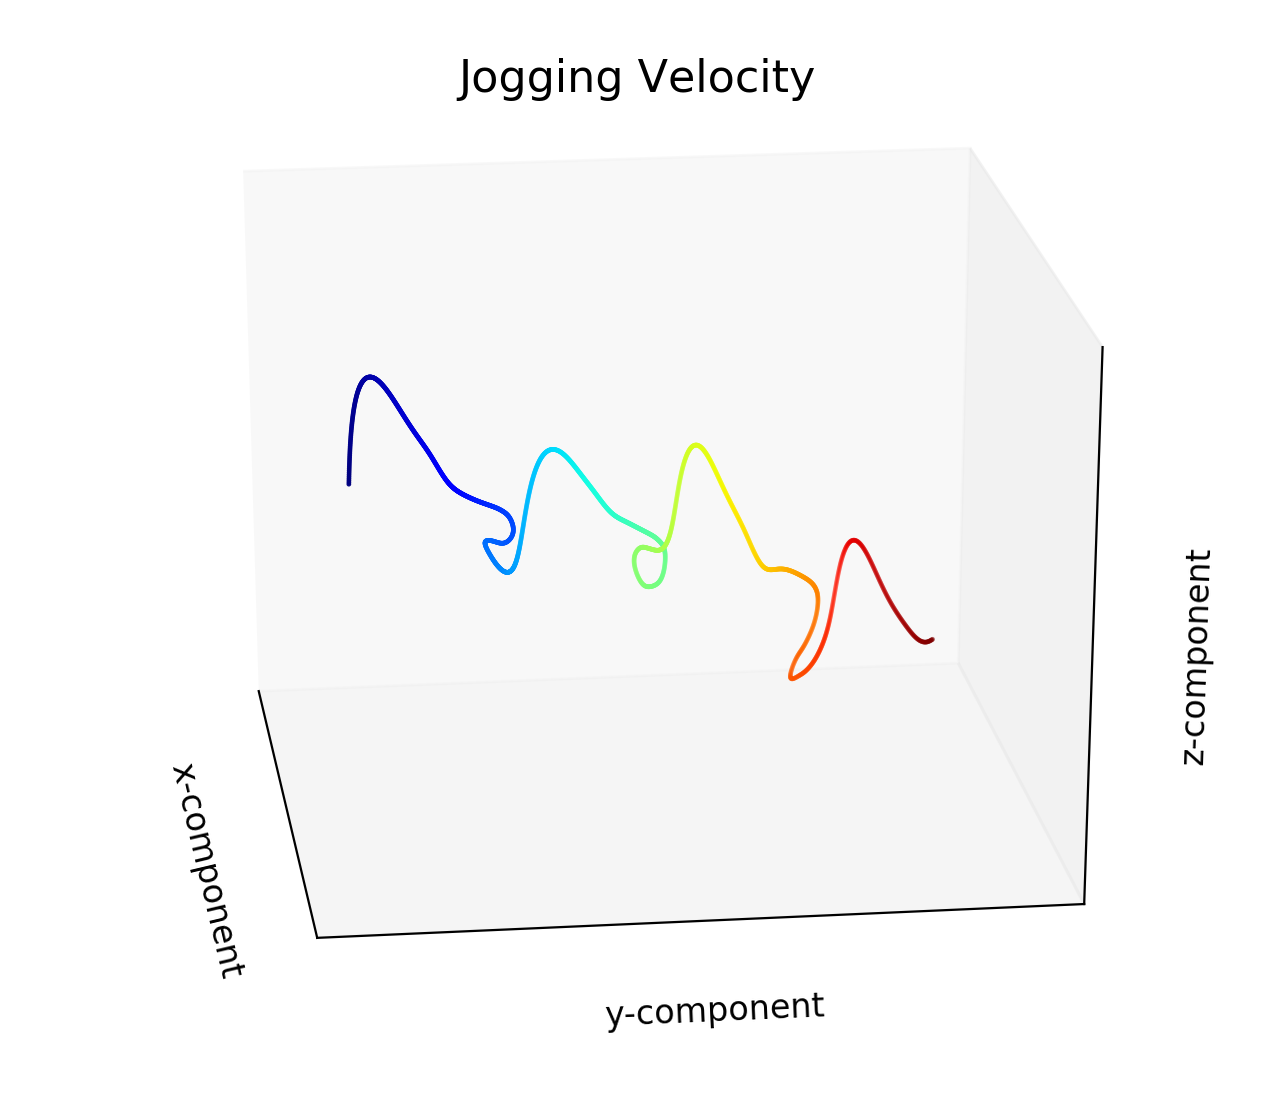
\includegraphics[width = 0.6 \textwidth]{images/comparisons/jogging.png}
    \caption{An example of a user's jogging accelerometer data integrated. Notice the inherent drift and quasi-periodic structure. The blue color represents time at $t = 0$ and the red represents time at $t = \SI{2.56}{\s}.$  }
    \label{fig:jogging_param}
\end{figure}

\subsection{Coordinate-Invariant Features}
\label{sub:coord_invar}
Perhaps we can create features based on torsion and curvature measurements for sub-segments of a single feature vector. We can take each of our accelerometer measurements. Since these are geometric quantities, they do not depend on any reference frame. So, for example, we can plot the magnitude of the torsion of the velocity to get a new feature that is independent of any coordinate system. Similarly, we can look at the magnitude of the torsion vector and get another, more distinct feature from the velocity. Both the torsion and curvature of a specific user is illustrated in Figure~\ref{fig:coord_inv} below.

\begin{figure}[ht]
\begin{subfigure}{.5\textwidth}
  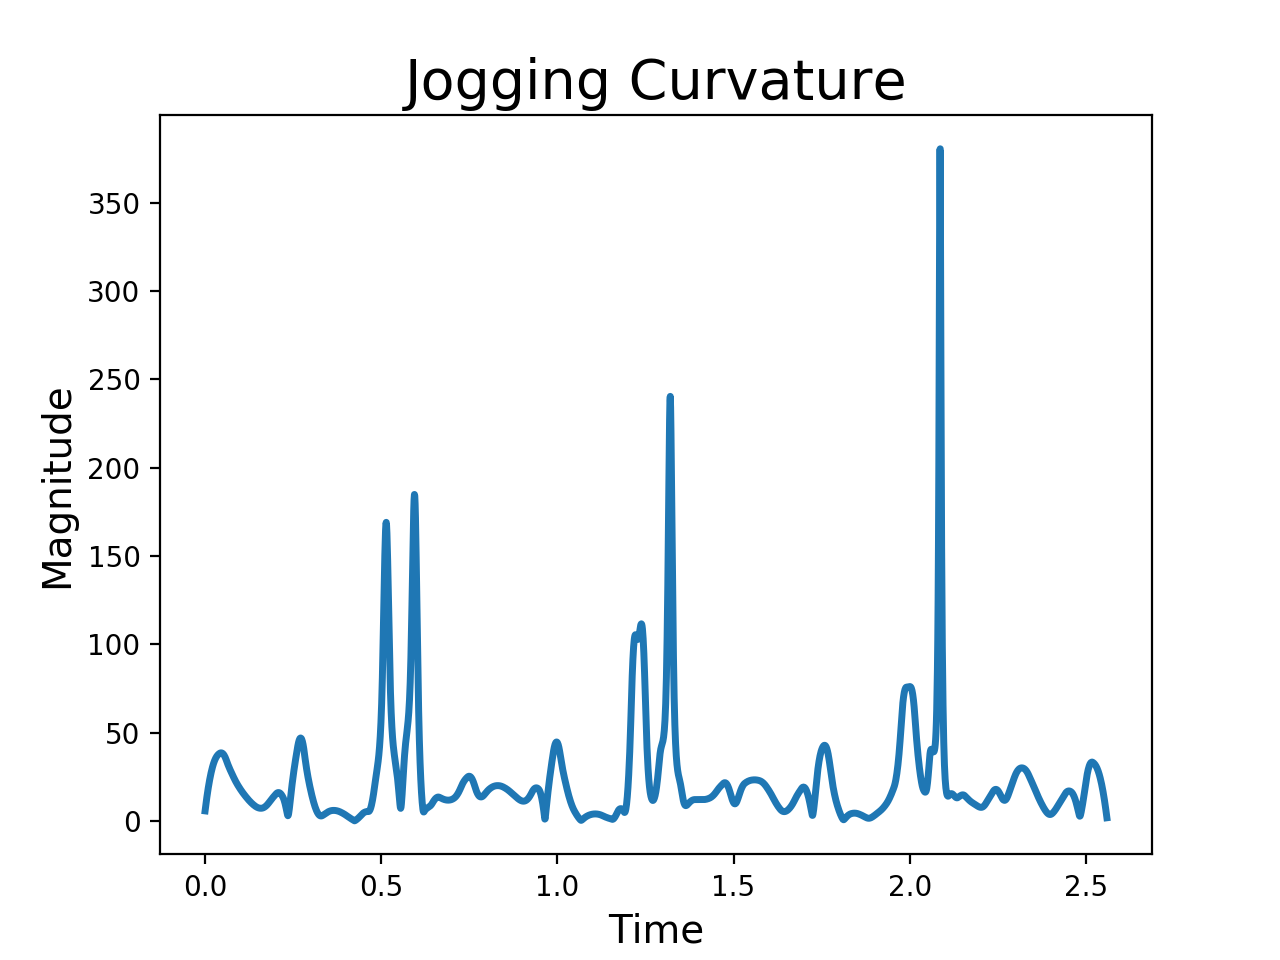
\includegraphics[width = 0.9\textwidth]{images/comparisons/jog_curv.png}
    \caption{Curvature.}
    \label{fig:curv}
\end{subfigure}
\begin{subfigure}{.5\textwidth}
    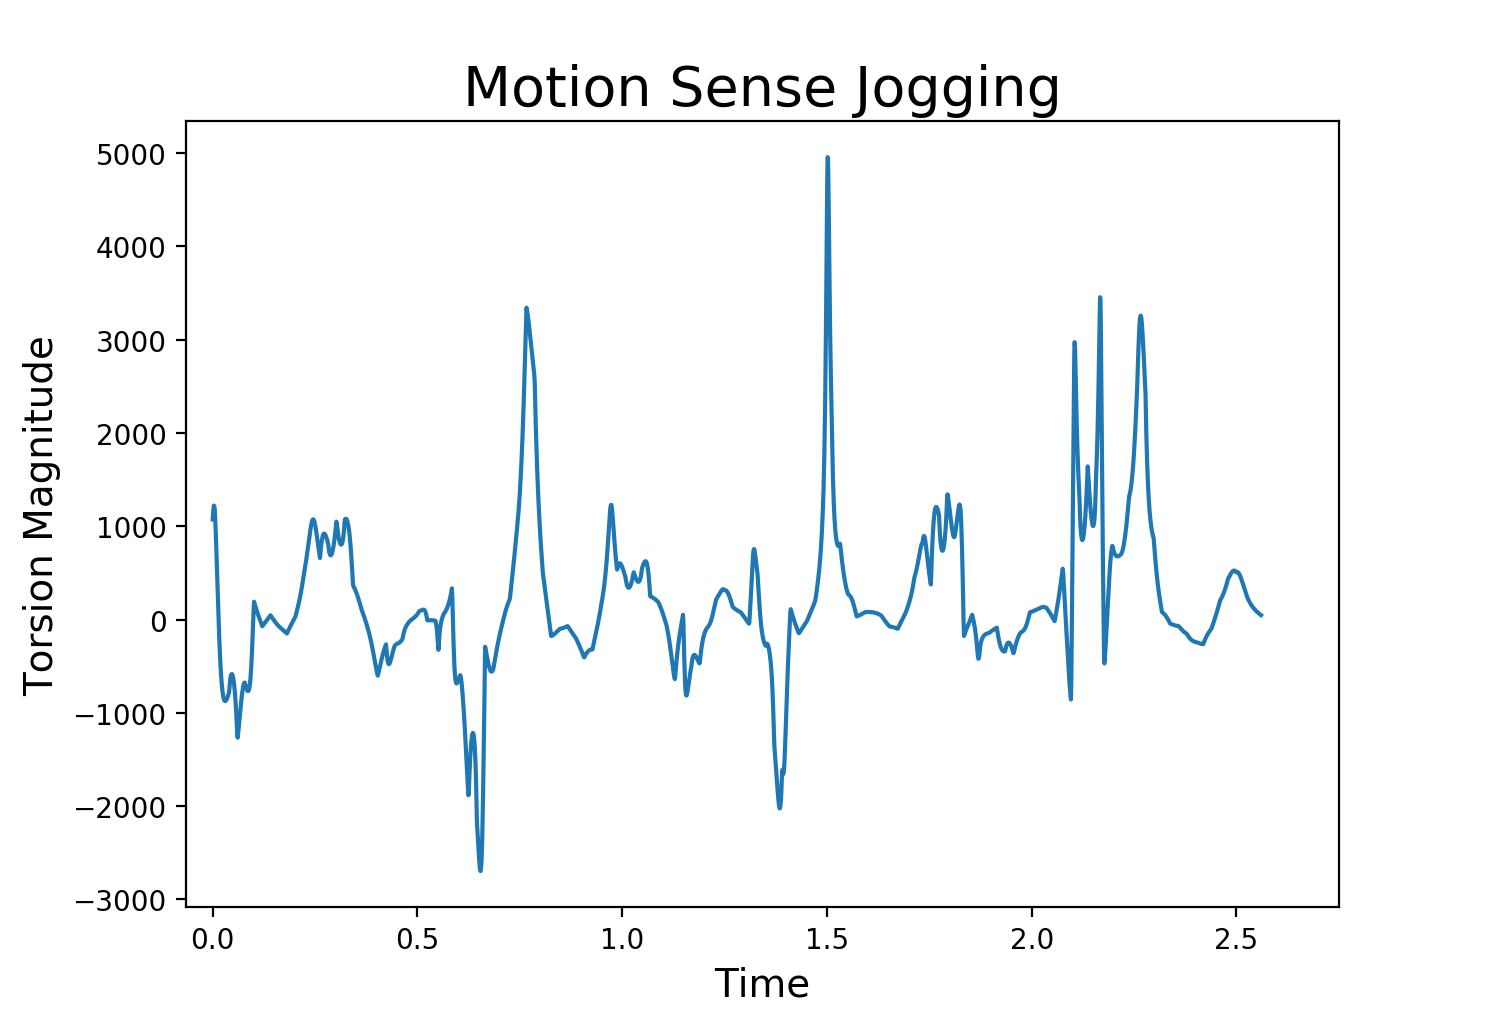
\includegraphics[width = \textwidth]{images/comparisons/jog_tor.png}
    \caption{Torsion.}
    \label{fig:tor}
\end{subfigure}
\caption{The magnitude of the torsion of velocity parameterized by time. This is a coordinate-invariant which is not dependent on the choice of axes.}
\label{fig:coord_inv}
\end{figure}

The periodic structure of Fig.~\ref{fig:coord_inv} implies that we should be looking for periodic patterns in our data, as it has important, activity-dependent information contained in it. This leads us to consider another type of feature---one that is time-invariant.
	

\begin{figure}[H]
\begin{subfigure}{.5\textwidth}
  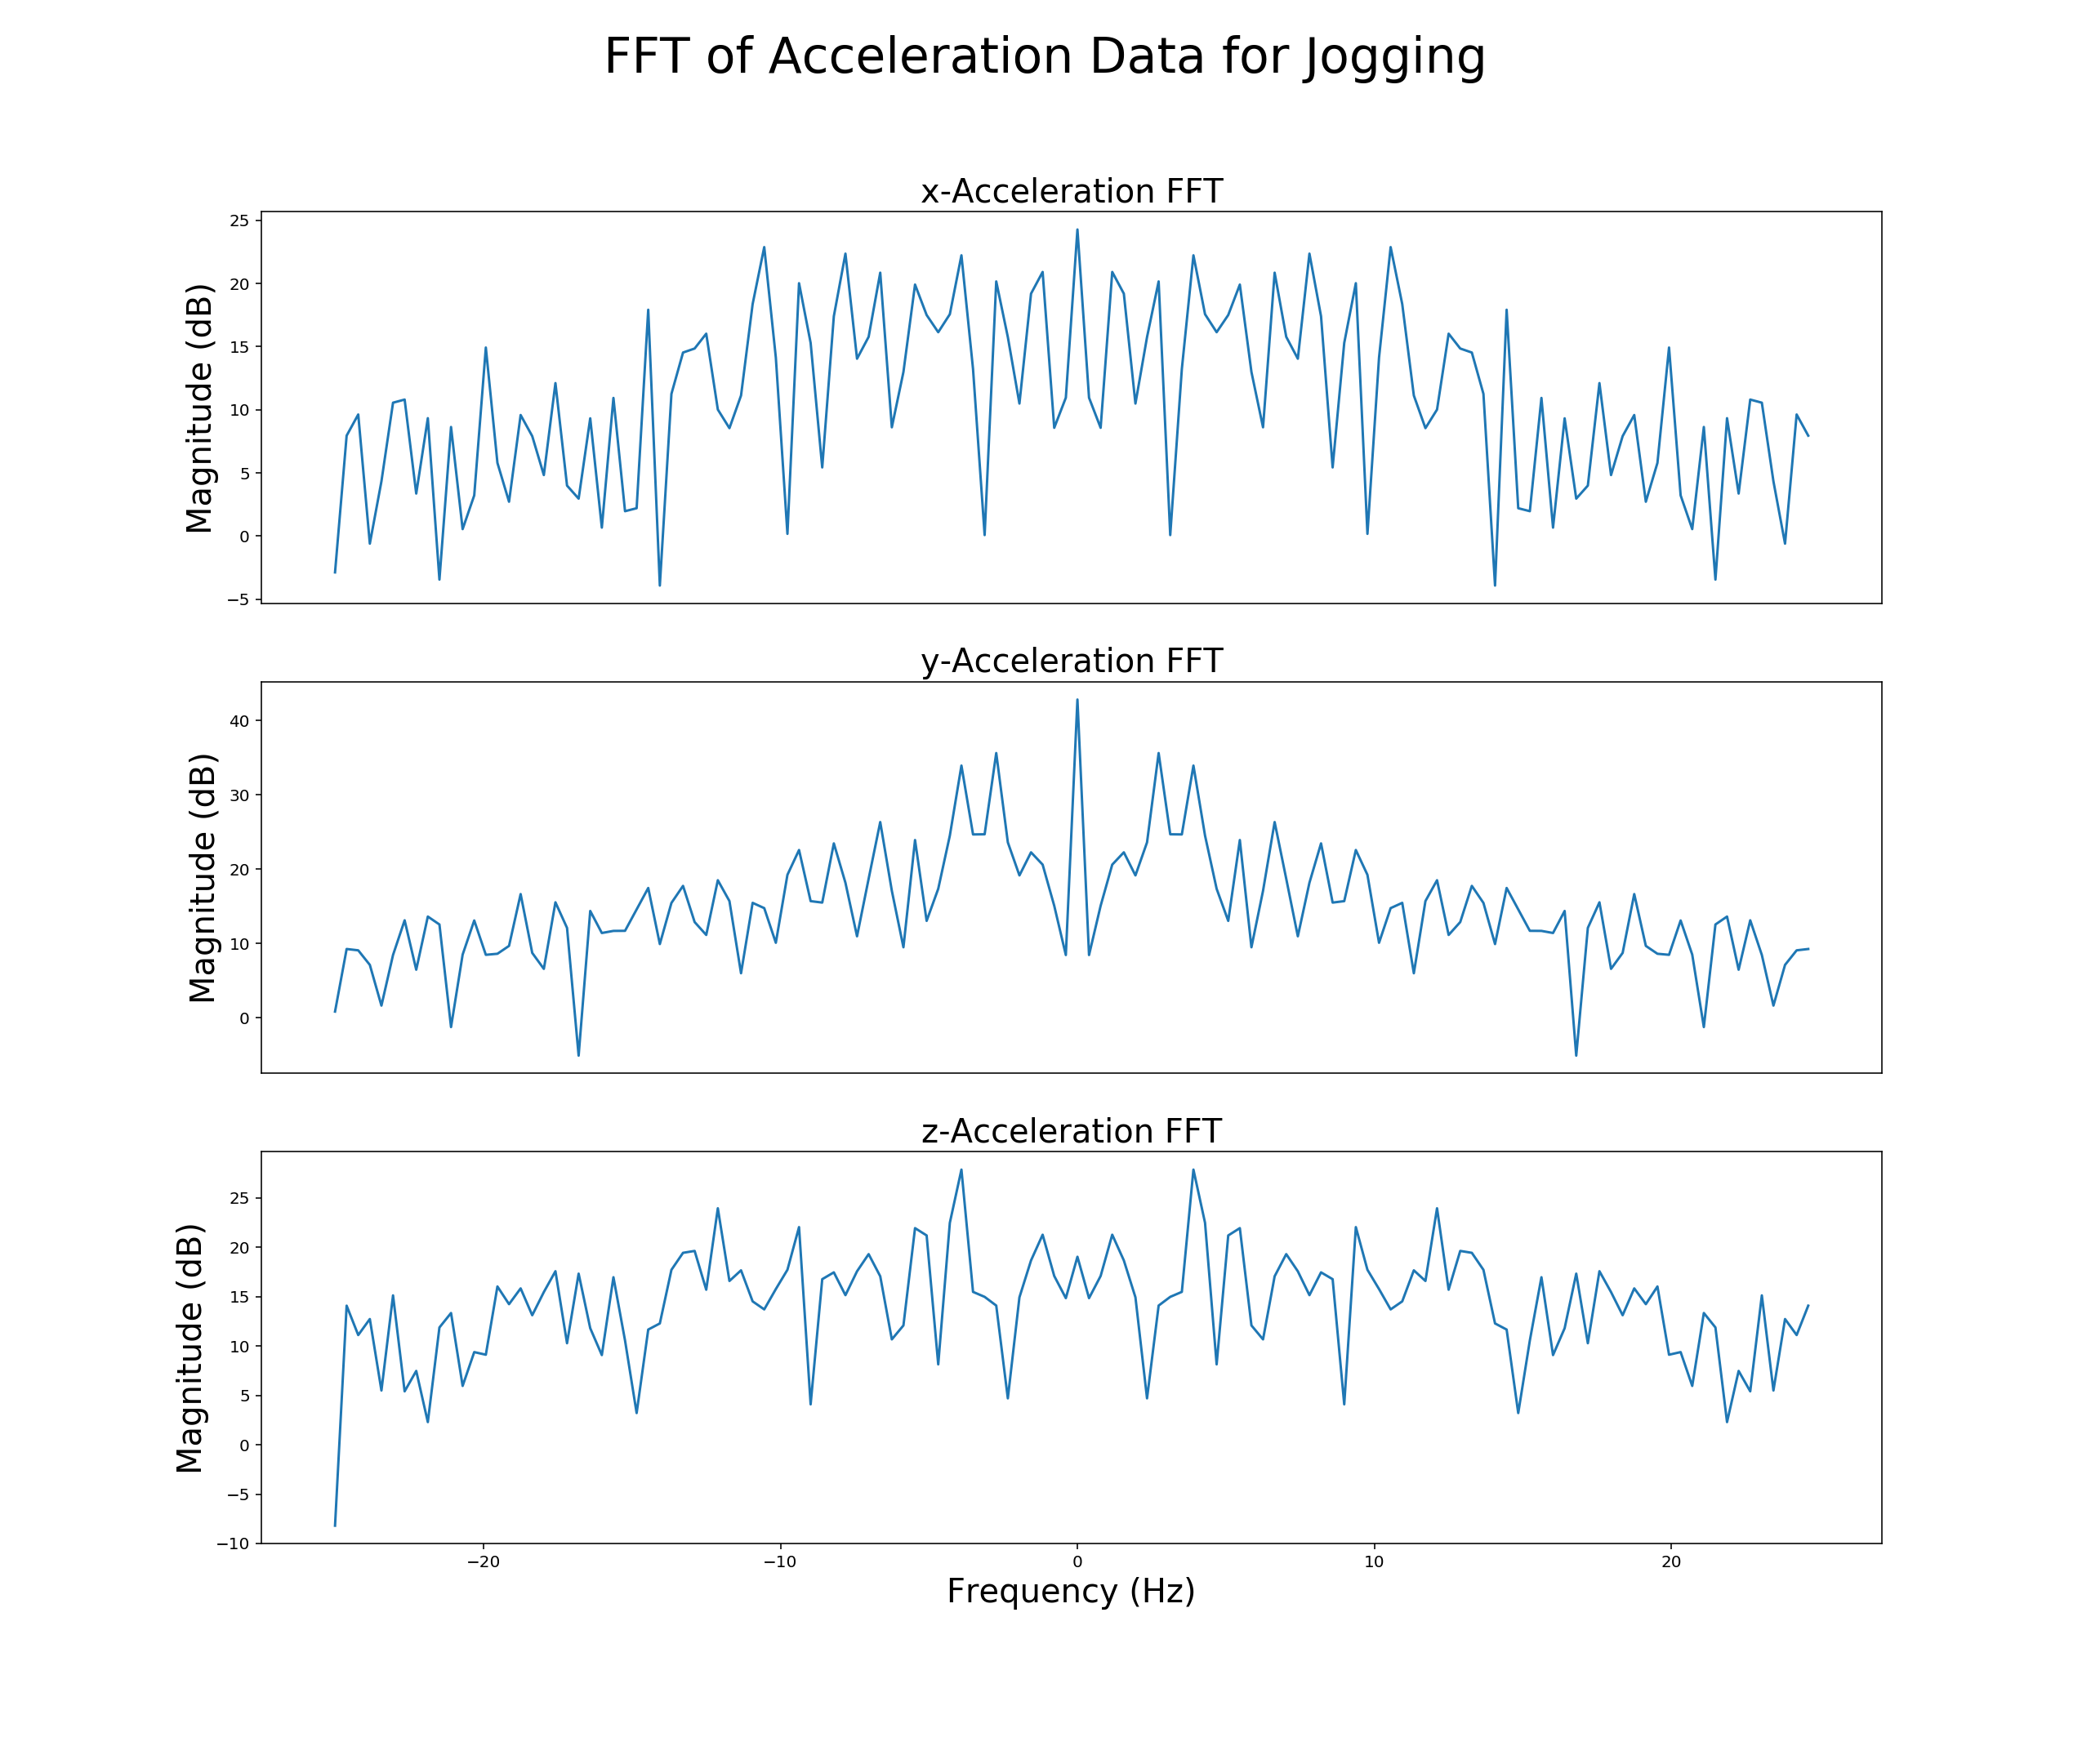
\includegraphics[width = 0.9\textwidth]{images/comparisons/JoggingFFT.png}
    \caption{FFT of a jogging feature vector.}
     \label{fig:jogFFT}
\end{subfigure}
\begin{subfigure}{.5\textwidth}
    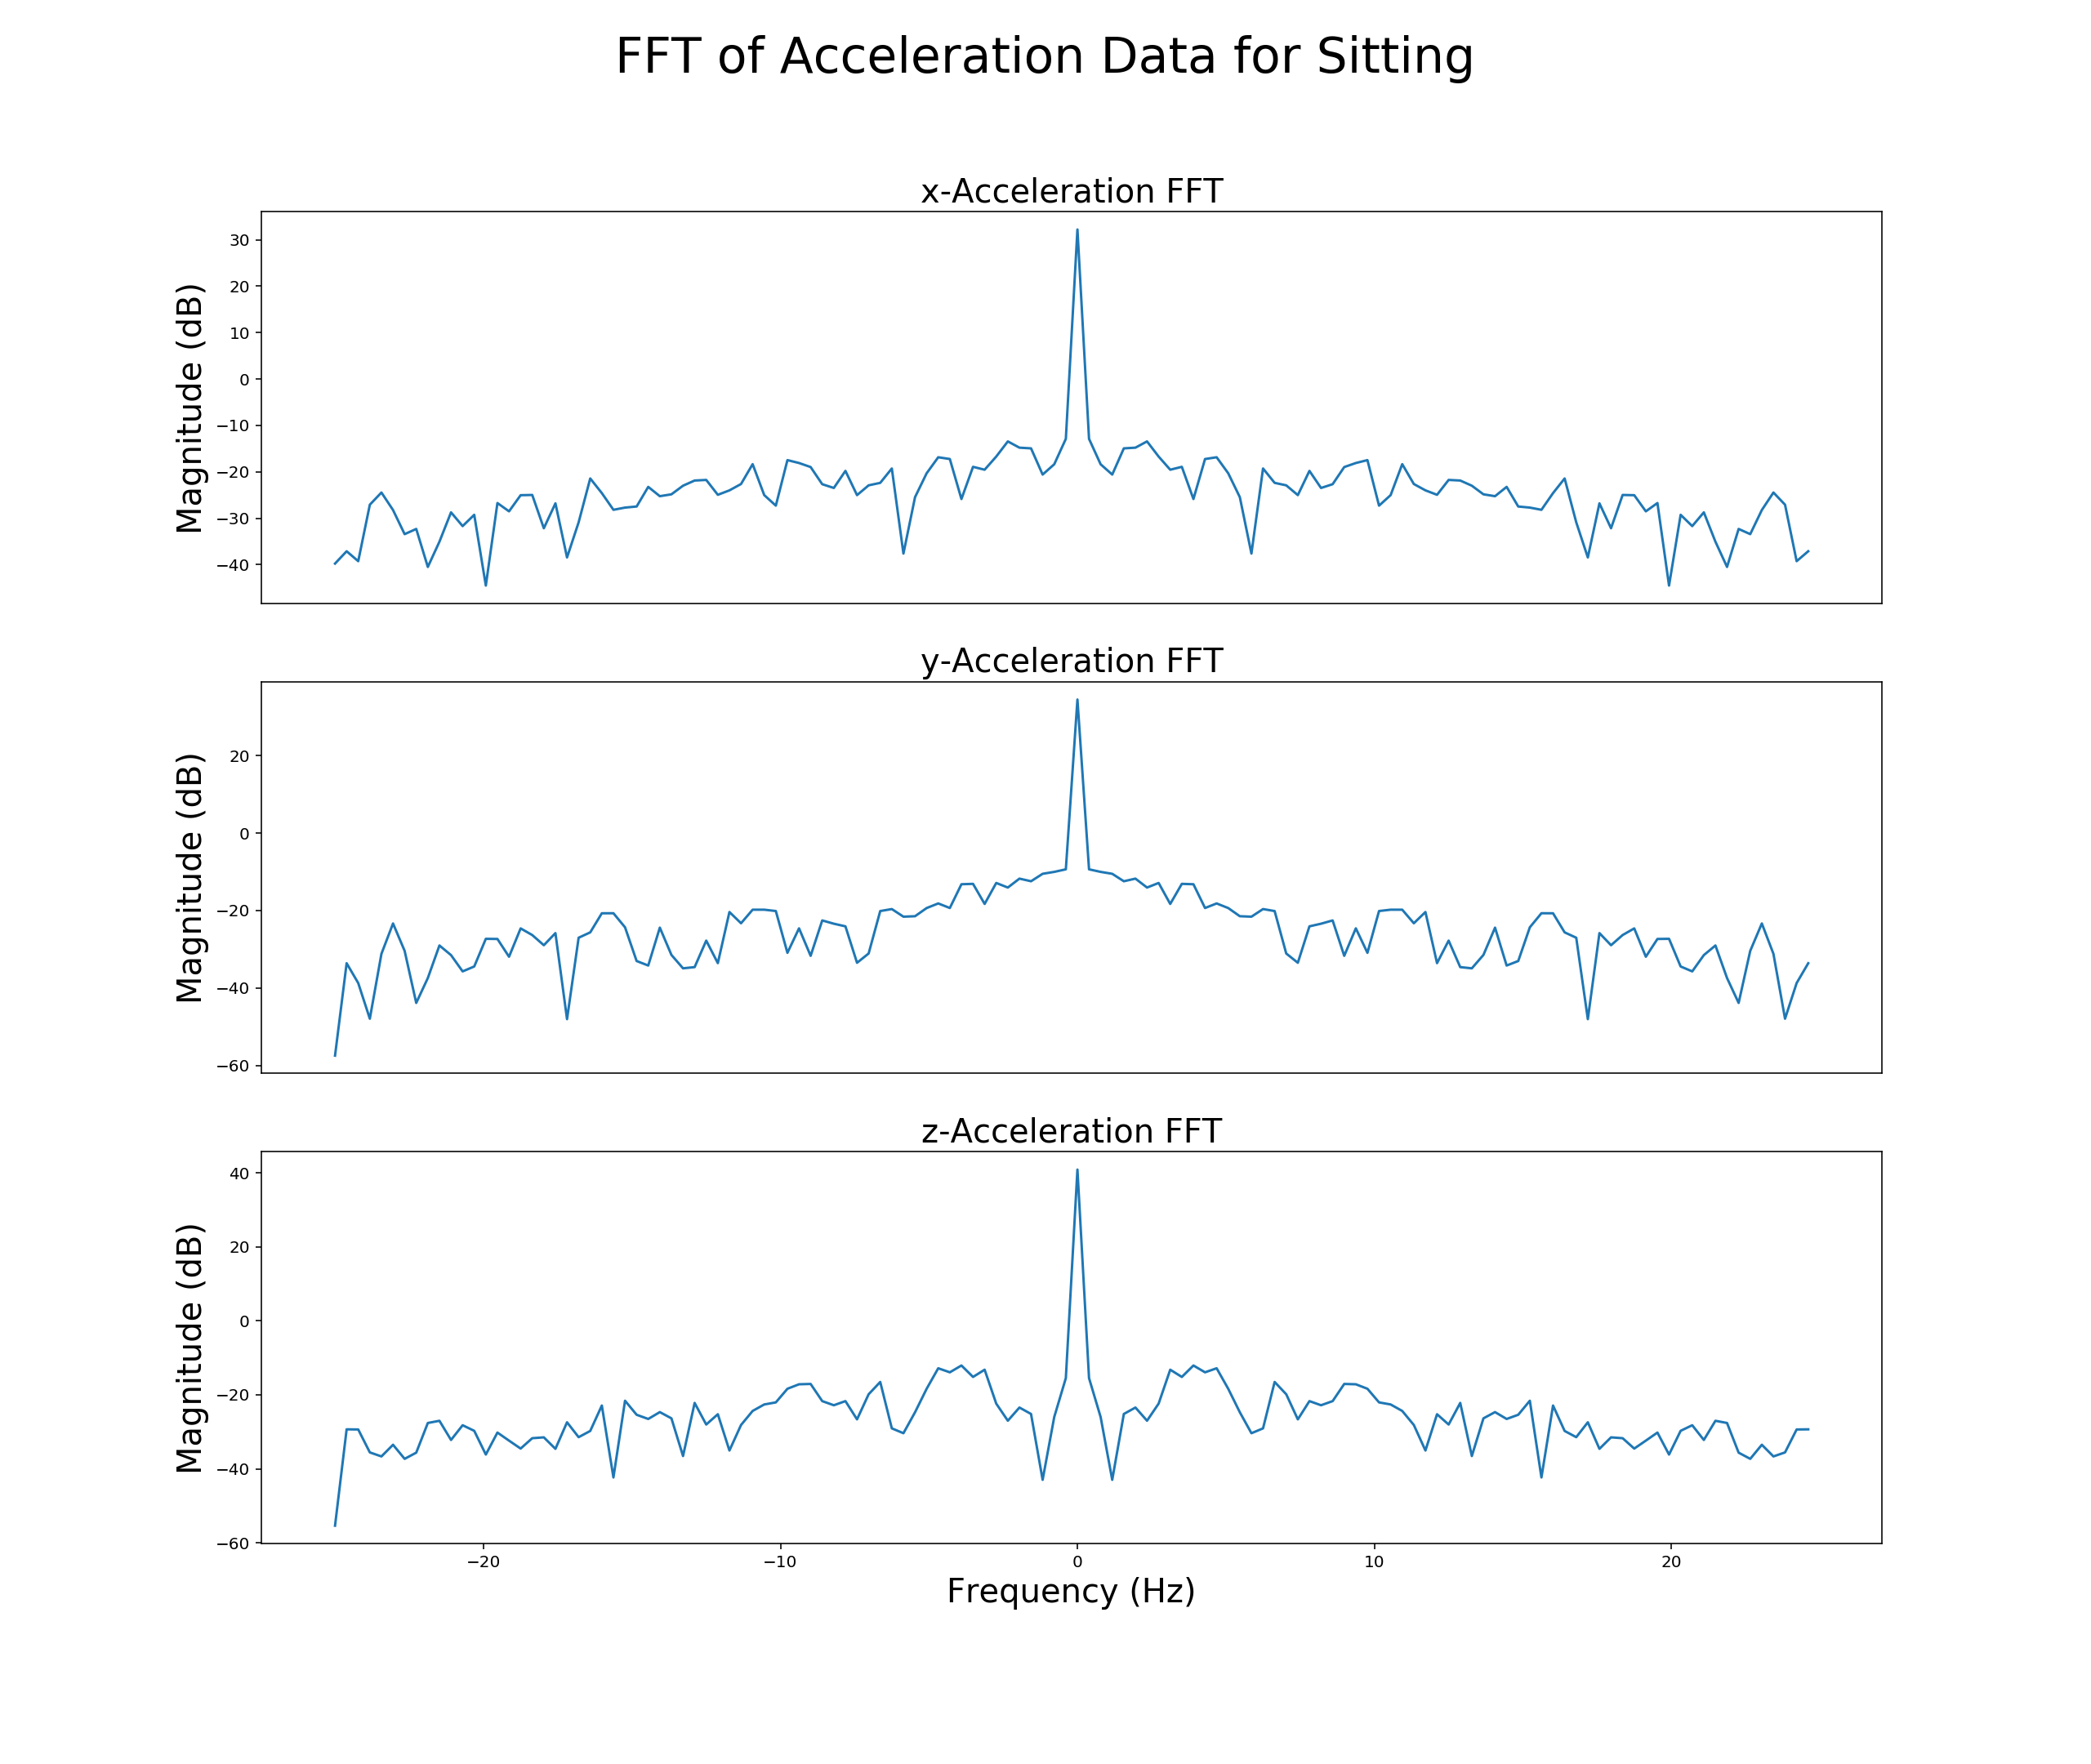
\includegraphics[width = 0.9 \textwidth]{images/comparisons/SittingFFT.png}
    \caption{FFT of a sitting feature vector.}
    \label{fig:sitFFT}
\end{subfigure}
\caption{The FFTs of the two aforementioned activities look very different. While sitting is primarily made up a DC component, due the lack of movement, the jogging signal has a variety of frequencies with large magnitudes.}
\label{fig:fft_comp}
\end{figure}


\begin{figure}[H]
\begin{subfigure}{.5\textwidth}
  \includegraphics[width = \textwidth]{images/hc_feats/ma/absAvgAcc_x.png}
    \caption{MobiAct}
    \label{fig:avg_abs_acc_x_ma}
\end{subfigure}
\begin{subfigure}{.5\textwidth}
    \includegraphics[width = \textwidth]{images/hc_feats/ms/absAvgAcc_x.png}
    \caption{MotionSense}
    \label{fig:avg_abs_acc_x_ms}
\end{subfigure}
\begin{subfigure}{.5\textwidth}
  \includegraphics[width = \textwidth]{images/hc_feats/ma/absAvgAcc_y.png}
    \caption{MobiAct}
    \label{fig:avg_abs_acc_y_ma}
\end{subfigure}
\begin{subfigure}{.5\textwidth}
    \includegraphics[width = \textwidth]{images/hc_feats/ms/absAvgAcc_y.png}
    \caption{MotionSense}
    \label{fig:avg_abs_acc_y_ms}
\end{subfigure}
\begin{subfigure}{.5\textwidth}
  \includegraphics[width = \textwidth]{images/hc_feats/ma/absAvgAcc_z.png}
    \caption{MobiAct}
    \label{fig:avg_abs_acc_z_ma}
\end{subfigure}
\begin{subfigure}{.5\textwidth}
    \includegraphics[width = \textwidth]{images/hc_feats/ms/absAvgAcc_z.png}
    \caption{MotionSense}
    \label{fig:avg_abs_acc_z_ms}
\end{subfigure}
\caption{Average Magnitude of Acceleration}
\label{fig:avg_abs_acc}
\end{figure}

		
\subsection{Time-Invariant Features}
\label{sub:time_invar}
	 
As shown in Fig.~\ref{fig:motionSense_grid}, the processed acceleration data is actually quite periodic, with the frequency of the signal changing for each activity. However, by including the raw accelerometer data in our feature vectors (in line with other researchers in the field), our classifier will be sensitive to where in the period of someones gait a time-window is centered on. By viewing the accelerometer data in the frequency domain instead of in the time domain, we could reduce the sensitivity to where an individual sample is centered. Researchers have previously have utilized discrete Fourier transform based features for accelerometer data \cite{ferrari2019hand}, although they stop short of directly using a power spectra in lieu of the time series. Figure~\ref{fig:fft_comp} shows a comparison of an FFT for jogging and sitting.

\subsection{Coordinate and Time Invariant Features}
\label{sub:coor_time_invar}

As stated in Sections~\ref{sub:coord_invar} and \ref{sub:time_invar}, there is likely to be significant gain from using coordinate and time invariant features. Figure~\ref{fig:coord_inv} shows that there is some periodicity within the coordinate invariant features of curvature and torsion. Thus, if we were to do the FFT of these features, we would then have features that are time and coordinate invariant.

\subsection{Hand-Crafted Features}
\label{sub:hc_feats}
Our coordinate- and time-invariant features aim to robustly describe how the phone moves. Such a description should be able to distinguish between activities with different structure --e.g.\ running vs.\ sitting or walking vs.\ sitting. However, we would expect this description to struggle at separating sitting from standing, where the distinguishing factor is not how the phone is moving, but what direction it is oriented. To capture this information, we created five hand-crafted features in addition to the torsion and curvature based features. These features aim to separate sedentary activities from active activities and to capture the orientation of a phone during a sedentary activity.  
\begin{figure}[ht]
\begin{subfigure}{.5\textwidth}
  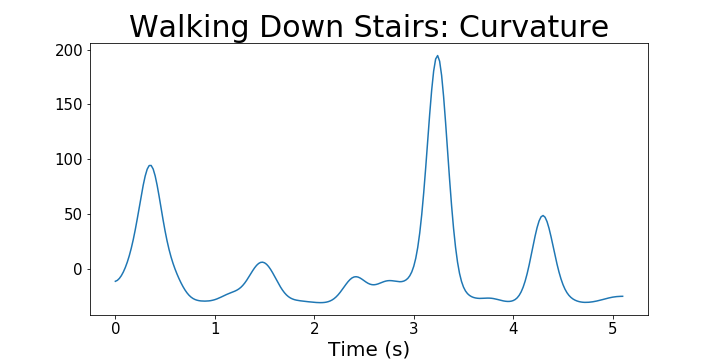
\includegraphics[width = \textwidth]{images/smooth/Walking Down Stairs curvature_ma.png}
    \caption{}
    \label{fig:walkdown_scurv}
\end{subfigure}
\begin{subfigure}{.5\textwidth}
    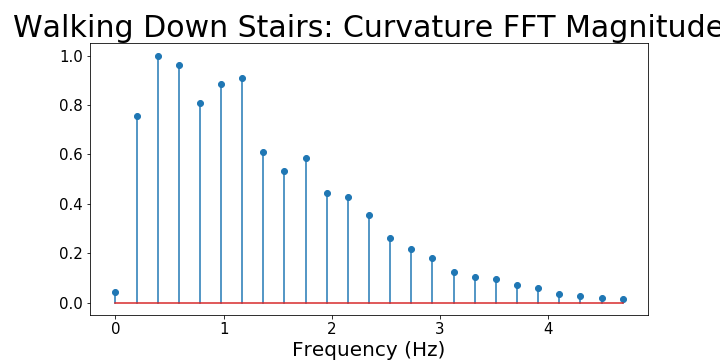
\includegraphics[width = \textwidth]{images/smooth/Walking Down Stairs curvatureFFT_ma.png}
    \caption{}
    \label{fig:walkdown_scur_fft}
\end{subfigure}
\begin{subfigure}{.5\textwidth}
  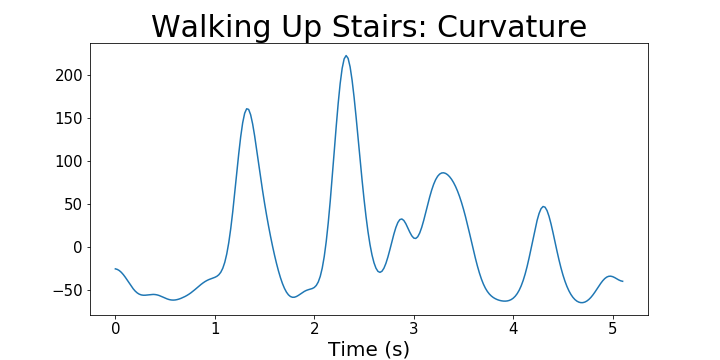
\includegraphics[width = \textwidth]{images/smooth/Walking Up Stairs curvature_ma.png}
    \caption{}
    \label{fig:walkup_scurv}
\end{subfigure}
\begin{subfigure}{.5\textwidth}
    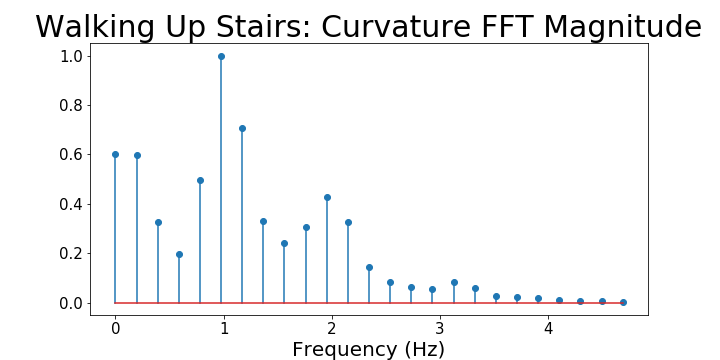
\includegraphics[width = \textwidth]{images/smooth/Walking Up Stairs curvatureFFT_ma.png}
    \caption{}
    \label{fig:walkup_scur_fft}
\end{subfigure}
\caption{An example of the smoothed values of curvature and the associated fast Fourier transform of the data for walking downstairs and upstairs. Comparing the FFT results around the \SI{1.2 }{\Hz} shows some of the largest differences between the two activities.}
\label{fig:curv_smooth}
\end{figure}

Our final feature vector consisted of:
\begin{enumerate}
    \item The power spectra of the fast Fourier transform of the magnitude of curvature of the parameterization of the acceleration as a function of time. Curvature, quite simply, is the measure of how much a curve deviates from a straight line. Its mathematical definition is \[ {\kappa} = \frac{\norm{\boldsymbol{\gamma}' \cross \boldsymbol{\gamma}''}}{\norm{\boldsymbol\gamma'}^3} \] where $\boldsymbol{\gamma} = (x(t), y(t), z(t))$. 
    
    In our case we are actually looking at the acceleration of the phone's body frame. Figure~\ref{fig:curv} shows that there is a highly periodic structure of the curvature's magnitude, and this is our reasoning for looking at the curvature in frequency space. In effect, this measures how quickly a phone changes direction in three-dimensional space. Due to the symmetry of FFTs, this accounts for 128 dimensions, however the high frequency components are negligible, so we restrict ourselves to looking at the first 25 components, corresponding to roughly \SIrange{0}{5}{\Hz}. Our actual process includes a Gaussian filter with $\sigma = $\SI{0.1}{s} to make our peaks smoother and remove as many of the sharp peaks as possible. Then we demeaned the curvature data before taking the FFT in order to reduce the DC component. Then we normalized the power spectra by the largest amplitude, and stored that value in our feature vector. This normalization was performed in order to have the same bounded range of frequency magnitudes between feature vectors. Figure~\ref{fig:curv_smooth} shows a nice illustration of a single result we had.  
    
    \item Similar to above, we use the magnitude of the FFT of the torsion of the three-dimensional acceleration curve. The torsion is the measure of how quickly a curve is twisting out of the plane of curvature---if it is twisting upwards from the plane of curvature, it is positive and it is negative if it is twisting outwards. The formula for torsion is given by \[ \tau = \frac{\det(\boldsymbol{\gamma}', \boldsymbol{\gamma}'', \boldsymbol{\gamma}''')}{\norm{\boldsymbol{\gamma}' \cross \boldsymbol{\gamma}''}^2}, \] where $\boldsymbol{\gamma}$ is the velocity parameterization again. This will hopefully account for changes in plane (e.g.\ walking up vs.\ down stairs). Just like curvature, we restricted ourselves to looking at the first 25 components, corresponding to roughly \SIrange{0}{5}{\Hz}. Our actual process includes a Gaussian filter with a window size of five to make our peaks smoother and remove as many of the sharp peaks as possible. Then we demeaned the curvature data before taking the FFT in order to reduce the DC component. Then we normalized the power spectra by the largest amplitude, and stored that value in our feature vector. This normalization was performed in order to have the same bounded range of frequency magnitudes between feature vectors. Figure~\ref{fig:tor_smooth} shows a nice illustration of a single result we had.
    
    \item Now we will look at the average acceleration vector $\expval{\vb{\abs{A}}} \equiv (\expval{\vb{\abs{A_x}}}, \expval{\vb{\abs{A_y}}}, \expval{\vb{\abs{A_z}}}$. This accounts for three of our 57 dimensions and will provide us with orientation data to distinguish sitting and standing as we expect standing will primarily be in the $A_y$ direction, hence the absolute value for an entire time series. Figure~\ref{fig:avg_abs_acc} shows a comparison between the MobiAct and MotionSense datasets for these features.
    
    \item The two remaining features are the average normalized demeaned acceleration (Eqn.~(\ref{eq:feat1})) as well as the standard deviation of the normalized demeaned acceleration (Eqn.~(\ref{eq:feat2})) as given below \begin{align}
        \expval{\abs{A - \expval{A}}} \label{eq:feat1} \\
        \mathrm{SD}({\abs{A - \expval{A}}})  \label{eq:feat2}
    \end{align}
    Figure~\ref{fig:avg_norm_demeaned_acc} and Figure~\ref{fig:std_norm_demeaned_acc} illustrate a comparison of these features between the MobiAct and MotionSense datasets.
\end{enumerate}
This, hopefully, will provide us with enough information to more accurately characterize human activities. 


\begin{figure}[ht]
\begin{subfigure}{.5\textwidth}
  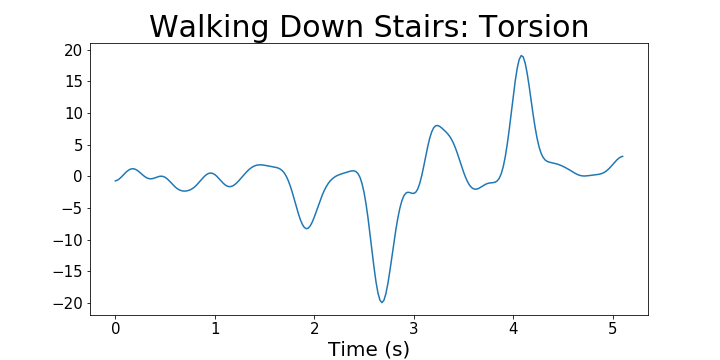
\includegraphics[width = \textwidth]{images/smooth/Walking Down Stairs torsion_ma.png}
    \caption{}
    \label{fig:walkdown_tor}
\end{subfigure}
\begin{subfigure}{.5\textwidth}
    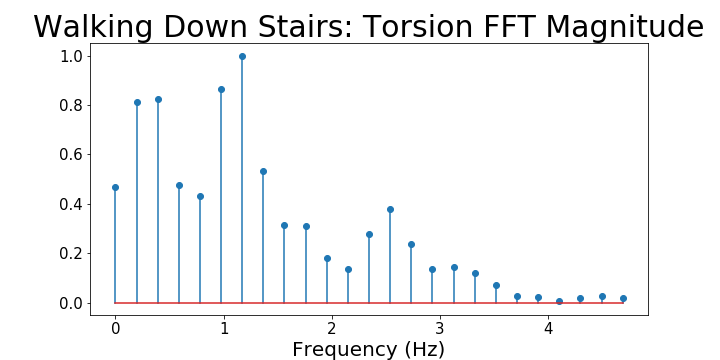
\includegraphics[width = \textwidth]{images/smooth/Walking Down Stairs torsionFFT_ma.png}
    \caption{}
    \label{fig:walkdown_tor_fft}
\end{subfigure}
\begin{subfigure}{.5\textwidth}
  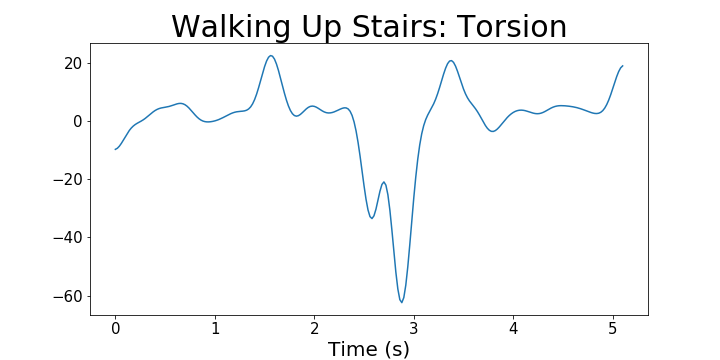
\includegraphics[width = \textwidth]{images/smooth/Walking Up Stairs torsion_ma.png}
    \caption{}
    \label{fig:walkup_stor}
\end{subfigure}
\begin{subfigure}{.5\textwidth}
    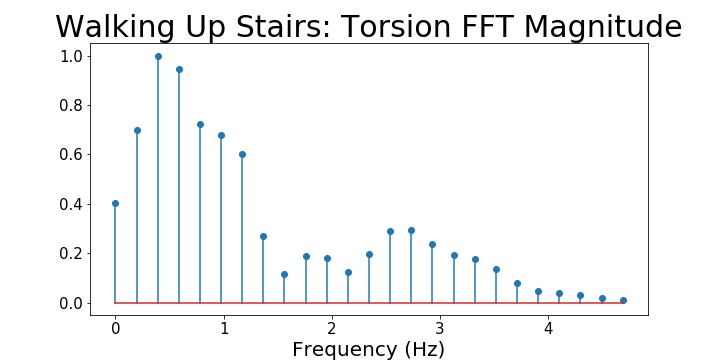
\includegraphics[width = \textwidth]{images/smooth/Walking Up Stairs torsionFFT_ma.png}
    \caption{}
    \label{fig:walkup_tor_fft}
\end{subfigure}
\caption{An example of the smoothed values of torsion and the associated fast Fourier transform of the data for walking downstairs and upstairs, two very similar behaviors. Comparing the FFT results around the \SI{1.2 }{\Hz} shows some of the largest differences between the two activities.}
\label{fig:tor_smooth}
\end{figure}


\begin{figure}[ht]
\begin{subfigure}{.5\textwidth}
  \includegraphics[width = \textwidth]{images/hc_feats/ma/avgNormAcc.png}
    \caption{MobiAct}
    \label{fig:avg_norm_demeaned_acc_ma}
\end{subfigure}
\begin{subfigure}{.5\textwidth}
    \includegraphics[width = \textwidth]{images/hc_feats/ms/avgNormAcc.png}
    \caption{MotionSense}
    \label{fig:avg_norm_demeaned_acc_ms}
\end{subfigure}
\caption{Average of the Normalized De-meaned Acceleration}
\label{fig:avg_norm_demeaned_acc}
\end{figure}

\begin{figure}[ht]
\begin{subfigure}{.5\textwidth}
  \includegraphics[width = \textwidth]{images/hc_feats/ma/stdNormAcc.png}
    \caption{MobiAct}
    \label{fig:std_norm_demeaned_acc_ma}
\end{subfigure}
\begin{subfigure}{.5\textwidth}
    \includegraphics[width = \textwidth]{images/hc_feats/ms/stdNormAcc.png}
    \caption{MotionSense}
    \label{fig:std_norm_demeaned_acc_ms}
\end{subfigure}
\caption{Standard Deviation of the Normalized Demeaned Acceleration}
\label{fig:std_norm_demeaned_acc}
\end{figure}




%as we saw earlier, our coordinate invariance can cause us to lose distinguishing features between activities, so we thought hand crafter would be a good idea. also paper showed that hand crafted helped a lot on their data set so we copy them kinda of



\subsection{Custom Data Collection}
\label{sub:og_data}

As shown in Table~\ref{tab:256naive}, the ExtraTrees classifier performed surprising well on the raw data for the cross dataset classification. If the phones were also orientated in the same direction (screen up vs screen down), then perhaps the cross data performance isn't so surprisingly. The drop from within dataset performance might simply be caused by the difference in the phone sensors. In addition, the \textsc{MobiAct} dataset was much more noisy than \textsc{MotionSense}, which could also contribute to the observed performance difference. 

If the \textsc{MobiAct} and \textsc{MotionSense} datasets
were taken with the phone in the same orientation, our personal dataset should perform similarly to the cross dataset results when our orientations match, but much worse when the orientations are completely opposite. In addition, if our classifier is truly coordinate invariant, we expect there to be no difference in performance between the two different orientation datasets that we collected. 


\subsection{Results of Hand-Crafted Features}
\label{sub:final_results}

Table ~\ref{tab:all_results_ms_ma} shows that our hand crafted features performed similarly to the raw data. However, the bulk of this performance was because of the 5 raw data based features; there was not a significant drop in performance for when we did not include the time and coordinate invariant based features. This leaves us to conclude that the frequencies of curvature and torsion of acceleration data are not beneficial for distinguishing the activities within the MotionSense and MobiAct datasets. However, we believe this is because these datasets are skewed heavily towards walking, jogging, sitting, and standing, and these activities can be effectively separated by simple measures of the magnitude of the motion and the orientation of the phone. Indeed we would not expect the curvature and torsion (invariant only) features to distinguish sitting and standing, which contributes to its seemingly poor performance. 

\begin{table}[H]
\centering
\caption{Summary of All Results}
\begin{tabular}{lcl}
\toprule
\multicolumn{1}{l}{\textbf{Raw Data}} & \multicolumn{1}{c}{\textbf{k-NN}} & \multicolumn{1}{c}{\textbf{Trees}}  \\ \midrule
\textsc{MotionSense} & 36.8\% & 68.6\% \\
\textsc{MobiAct}     & 44.3\% & 77.0\% \\
\toprule 
%%
\multicolumn{1}{l}{\textbf{All Custom}} & \multicolumn{1}{c}{\textbf{k-NN}} & \multicolumn{1}{c}{\textbf{Trees}}  \\ \midrule 
\textsc{MotionSense} & 37.5\% & 68.1\% \\
\textsc{MobiAct}     & 41.2\% & 69.6\% \\
\toprule 
%%
\multicolumn{1}{l}{\textbf{Invariant Only}} & \multicolumn{1}{c}{\textbf{k-NN}} & \multicolumn{1}{c}{\textbf{Trees}}  \\ \midrule
\textsc{MotionSense} & 37.5\% & 38.2\% \\
\textsc{MobiAct}     & 41.2\% & 40.2\% \\
\toprule 
%%
\multicolumn{1}{l}{\textbf{Five Features}} & \multicolumn{1}{c}{\textbf{k-NN}} & \multicolumn{1}{c}{\textbf{Trees}}  \\ \midrule
\textsc{MotionSense} & 71.2\% & 71.7\% \\
\textsc{MobiAct}     & 63.0\% & 63.1\% \\
\bottomrule
\end{tabular}
\label{tab:all_results_ms_ma}
\end{table}

To test whether our features are actually orientation invariant, we performed an analysis using custom data. We each performed the same activities twice: once with our phone facing out, the other with our phone facing in (both were done with the bottom of the phone at the bottom of a front pocket). We again compared the results of only using raw data, all of our hand-crafted features, only the time and coordinate invariant features, and only the raw data-based features. In this case, our coordinate invariant features (curvature and torsion) alone were able to outperform the raw data. Using all of the handcrafted features performed better, while the five raw data based features alone performed the best. 

This dataset is essentially a toy problem: i.e.\ the same person performs the same activity with the only change being the phone's orientation. That being said, it illustrates that the curvature and torsion based features can capture the essence of how the phone moves in an orientation independent manner, and it is able to outperform the raw data for this small dataset. For the larger datasets, the sheer volume of data is enough to overcome this limitation for the raw data, or it may be that the datasets contain samples of the phone at different orientations. Regardless, we believe that our custom data clearly indicates the potential of our technique.

\begin{table}[ht]
\centering
\caption{Experiments on Phone Orientation in Pocket, Across Datasets}
\begin{tabular}{lcl}
\toprule
\multicolumn{1}{l}{\textbf{Raw Data}} & \multicolumn{1}{c}{\textbf{k-NN}} & \multicolumn{1}{c}{\textbf{Trees}}  \\ \midrule
\textsc{Inwards} & 25.7\% & 69.2\% \\
\textsc{Outwards}     & 25.6\% & 59.7\% \\
\toprule 
%%
\multicolumn{1}{l}{\textbf{All Custom}} & \multicolumn{1}{c}{\textbf{k-NN}} & \multicolumn{1}{c}{\textbf{Trees}}  \\ \midrule 
\textsc{Inwards} & 73.7\% & 96.5\% \\
\textsc{Outwards}     & 74.0\% & 95.3\% \\
\toprule 
%%
\multicolumn{1}{l}{\textbf{Invariant Only}} & \multicolumn{1}{c}{\textbf{k-NN}} & \multicolumn{1}{c}{\textbf{Trees}}  \\ \midrule
\textsc{Inwards} & 73.7\% & 72.0\% \\
\textsc{Outwards}     & 74.0\% & 76.4\% \\
\toprule 
%%
\multicolumn{1}{l}{\textbf{Five Features}} & \multicolumn{1}{c}{\textbf{k-NN}} & \multicolumn{1}{c}{\textbf{Trees}}  \\ \midrule
\textsc{Inwards} & 97.0\% & 97.4\% \\
\textsc{Outwards}     & 96.8\% & 97.7\% \\
\bottomrule
\end{tabular}
\label{tab:in_out}
\end{table}

While these raw data based features were important for cross dataset analysis, we wanted to see if they were equally as powerful for within dataset analysis for activity recognition between users. The difference within a single dataset being that all data is gathered with the same device and the definition of each activity is consistent. Table ~\ref{tab:ms_ms_user_5} shows that these raw features do perform nearly as well as the raw data for cross validation by user within a dataset for extra trees, and they increase performance for the k-NN. 


\begin{figure}[ht]
  \includegraphics[width = \textwidth]{images/confusion/conf_all.png}
    \caption{Confusion matrices for the four cross dataset trials. The trial with the best performance for each activity is highlighted in red.}
    \label{fig:conf_all}
\end{figure}

\begin{table}[ht]
\centering
\caption{Intradataset Results: Cross Validation by User}
\begin{tabular}{lcl}
\toprule
\multicolumn{1}{l}{\textbf{Raw Data}} & \multicolumn{1}{c}{\textbf{k-NN}} & \multicolumn{1}{c}{\textbf{Trees}}  \\ \midrule
\textsc{MotionSense} & 73.8\% & 83.3\% \\
\textsc{MobiAct}     & 92.2\% & 94.1\% \\
\toprule
%%
\multicolumn{1}{l}{\textbf{Five Features}} & \multicolumn{1}{c}{\textbf{k-NN}} & \multicolumn{1}{c}{\textbf{Trees}}  \\ \midrule
\textsc{MotionSense} & 81.3\% & 79.4\% \\
\textsc{MobiAct}     & 92.4\% & 92.0\% \\
\bottomrule
\end{tabular}
\label{tab:ms_ms_user_5}
\end{table}



In addition to aggregate accuracy scores, it is also helpful to investigate which activities were classified. Figure~\ref{fig:conf_all} shows the confusion matrices for our different trials. In all cases, the classifier had difficulty distinguishing between walking, walking upstairs, and walking downstairs. This shouldn't be surprising when we compare these results to Figs.~\ref{fig:avg_norm_demeaned_acc_ma}~and~\ref{fig:avg_norm_demeaned_acc_ms}. Our hope was that the coordinate invariant Fourier transforms of curvature and torsion would be able to distinguish slight subtleties in these motions. However, it was unable to do so reliably. This is likely because there is a large difference between the amount of data for these activities. The confusion matrices show that walking and standing have an order of magnitude more data than the other activities. A more fair trial would be to train on a subset of the dataset that contains the same number of samples for each activity.

\subsection{Combined Raw Data and All Custom Features}

Since both our custom features as well as the raw data performed similarly, we decided to try and combine all of the information for our classifier to train on. The results were in line with what we would get with either just the raw data or just the custom features. The extra dimensionality added may have inhibited performance.  Table~\ref{tab:errything} summarizes these results.

\begin{table}[ht]
\centering
\caption{Raw Data and All Custom Features}
\toprule
%%
\multicolumn{1}{l}{\textbf{Raw + Custom}} & \multicolumn{1}{c}{\textbf{k-NN}} & \multicolumn{1}{c}{\textbf{Trees}}  \\ \midrule
\textsc{MotionSense} & 40.1\% & 66.3\% \\
\textsc{MobiAct}     & 40.1\% & 72.3 \% \\
\bottomrule
\end{tabular}
\label{tab:errything}
\end{table}


\subsection{A Digression on Dimensionality}

While our classifier's results were on par with the performance of merely training on the raw data, we would like to point out the drastic reduction in dimensionality our five-feature classifier achieved. With the raw data, we fed in the accelerometer data at 256 times, each of which has three components ($a_x,a_y,a_z$) for a total of 768 dimensions. This is more than a 150-fold decrease in dimensionality while achieving the same essentially the same results. This, in itself, is mildly impressive.